\usepackage {picins}
\section{Einleitung}
\begin{description}
	In Wohngemeinschaften oder kleineren Wohnungen ist es oft nicht möglich Kleidung auf Wäscheständern oder -Leinen zu trocknen. Die Bewohner weichen auf den Keller oder Dachboden aus. In diesen Fällen ist die Wäsche nicht direkt überwachbar und eine genaue Abschätzung, wann die Wäsche trocken ist, ist kaum möglich. <br/>
Um die Trocknung der Wäsche im Auge zu behalten haben wir DryR entwickelt: <br\>
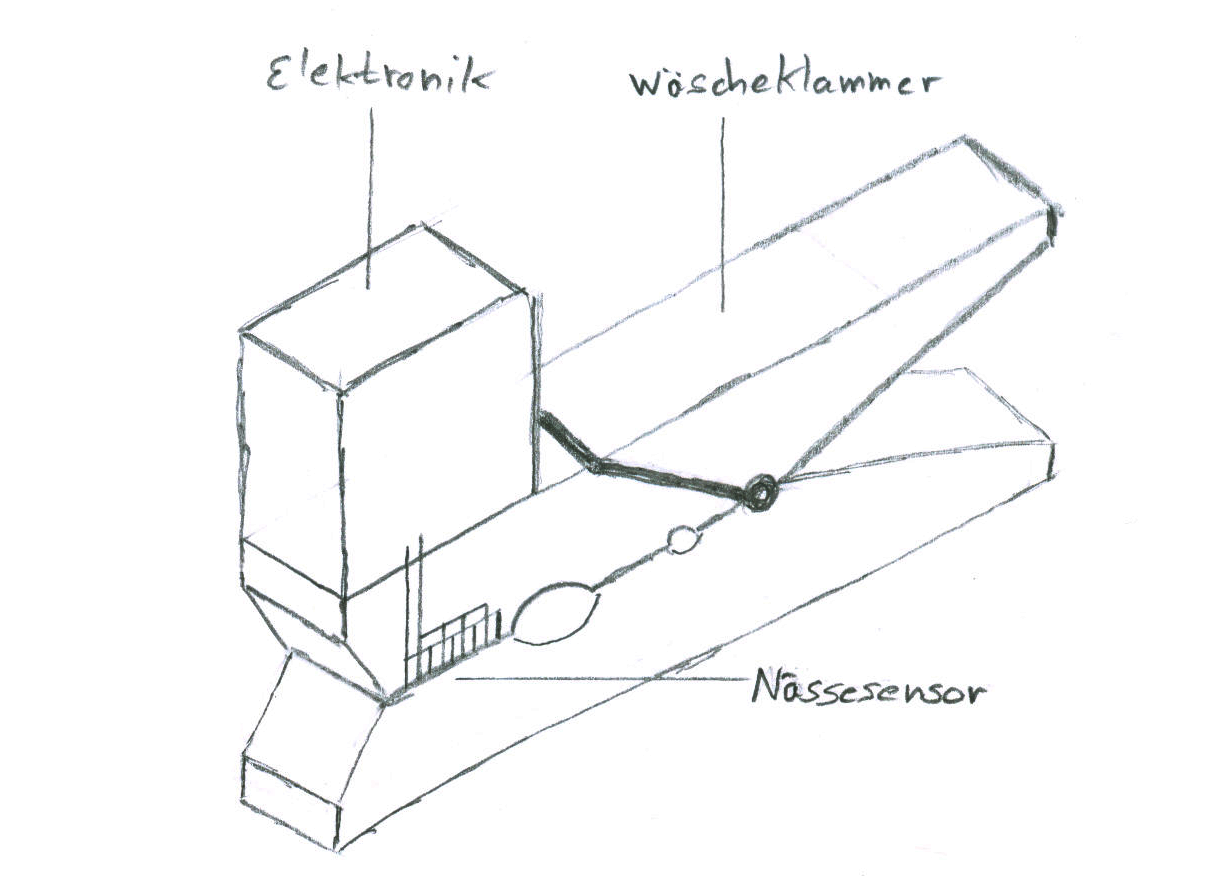
\includegraphics[width=0.7\textwidth]{01-klammer.png} <br\>
Ein Sensor der die Feuchtigkeit der Wäsche überwacht und in einer App anzeigt.

\end{description}
